
\documentclass[11pt]{article}
\usepackage[letterpaper, margin=1in]{geometry} 
\usepackage{hyperref}
\usepackage[leftcaption]{sidecap}
\sidecaptionvpos{figure}{c} %position side caption
\usepackage{lineno}
\usepackage{lipsum}
\usepackage{indentfirst}
\usepackage{pdflscape}
\usepackage{color}
\usepackage{multirow}
\usepackage[utf8]{inputenc}
\usepackage{array}
	\newcounter{rowno}
	\setcounter{rowno}{0}
\usepackage{booktabs}
\usepackage[pdftex]{graphicx}  
\usepackage{caption}
\usepackage{natbib}
\usepackage{authblk}
\usepackage[table]{xcolor} %for table line color alteration
\usepackage{subscript}
\usepackage{longtable}
\usepackage{fancyhdr}
	\renewcommand{\headrulewidth}{0pt}
	\rfoot{\thepage}
\fancyhf{}
\renewcommand{\headrulewidth}{0pt}

\pagestyle{fancy}

\begin{document}

\centering{Table S1: Accessions of \emph{Zea mays} ssp. \emph{mexicana} (RIMME) and \emph{Zea mays} ssp. \emph{parviglumis} (RIMPA) sampled. RIHY is a \emph{Z. mays} ssp. \emph{parviglumis} and \emph{Zea mays} ssp. \emph{mays} hybrid.}

% Appendix S1. Parv and mex samples 
\begin{scriptsize}  % Switch from 12pt to 11pt; otherwise, table won't fit
\rowcolors{1}{gray!25}{white}
\begin{longtable}{>{\stepcounter{rowno}}cccccc}
\hiderowcolors
\hline
\multicolumn{1}{c}{\textbf{Accession}} & \multicolumn{1}{c}{\textbf{USDA ID}} & \multicolumn{1}{c}{\textbf{Population}} & \multicolumn{1}{c}{\textbf{Alleles Sampled}} & \multicolumn{1}{c}{\textbf{\emph{Hopscotch} Freq.}} & \multicolumn{1}{c}{\textbf{No \emph{Hopscotch} Freq.}} \\
\hline
\endhead
\showrowcolors
    RIHY0009 & N/A   & N/A   & 2     & 0.5   & 0.5 \\
    RIMME0006 & PI 566673 & Durango & 2	& 0 & 1 \\
    RIMME0007 & PI 566680 & Guanajuato & 2 & 0 & 1 \\
    RIMME0008 & PI 566681 & Michoacan & 2 & 0 & 1 \\
    RIMME0009 & PI 566682 & Distrito Federal & 2 & 0 & 1 \\
    RIMME0011 & PI 566685 & Mexico & 2     & 0     & 1 \\
    RIMME0014 & Ames 28398 & TIL25 Jalisco  & 6     & 0     & 1 \\
    RIMME0017 & Ames 699874 & Ayotlan & 8     & 0     & 1 \\
    RIMME0021 & N/A   & El Porvenir & 69    & 0.17 & 0.83 \\
    RIMME0026 & N/A   & Opopeo & 42    & 0.07 & 0.93 \\
    RIMME0028 & N/A   & Puruandiro & 28    & 0.04 & 0.96 \\
    RIMME0029 & N/A   & Ixtlan & 35    & 0     & 1 \\
    RIMME0030 & N/A   & San Pedro & 27    & 0     & 1 \\
    RIMME0031 & N/A   & Tenango del Aire & 25    & 0.08  & 0.92 \\
    RIMME0032 & N/A   & Nabogame & 24    & 0     & 1 \\
    RIMME0033 & N/A   & Puerta Encantada & 25    & 0     & 1 \\
    RIMME0034 & N/A   & Santa Clara & 23    & 0     & 1 \\
    RIMME0035 & N/A   & Xochimilco & 25    & 0     & 1 \\
    RIMPA0001 & Ames 21786 & El Salado & 4     & 0     & 1 \\
    RIMPA0003 & Ames 21789 & Mazatlan & 8 & 0.13 & 0.87 \\
    RIMPA0017 & Ames 21814  & N/A   & 4     & 0     & 1 \\
    RIMPA0019 & Ames 21826 & El Salado & 2     & 0.50   & 0.50 \\
    RIMPA0029 & Ames 21853 & N/A   & 2     & 0.50   & 0.50 \\
    RIMPA0031 & Ames 21856 & N/A   & 2     & 0.5   & 0.5 \\
    RIMPA0035 & Ames 21889 & Jalisco & 4     & 0     & 1 \\
    RIMPA0040 & PI 384063 & Mexico & 4     & 0     & 1 \\
    RIMPA0042 & PI 384065 & Guerrero & 4     & 0.25  & 0.75 \\
    RIMPA0043 & PI 384066 & Guerrero & 4     & 0     & 1 \\
    RIMPA0045 & PI 384071 & Guerrero & 4     & 0     & 1 \\
    RIMPA0055 & Ames 28399 & TIL01, Michoacan & 2     & 0     & 1 \\
    RIMPA0056 & Ames 28400 & TIL03 Jalisco & 2     & 0.50   & 0.50 \\
    RIMPA0057 & Ames 28401 & TIL06 Guerrero & 2     & 0.50   & 0.50 \\
    RIMPA0058 & N/A   & N/A   & 4     & 0.50   & 0.50 \\
    RIMPA0059 & N/A   & N/A   & 4     & 1     & 0 \\
    RIMPA0060 & Ames 28404 & TIL10 Guerrero & 2     & 0     & 1 \\
    RIMPA0061 & Ames 28405 & TIL11 Nayarit & 4     & 0.5   & 0.5 \\
    RIMPA0062 & Ames 28406 & TIL14 Jalisco & 4     & 0.5   & 0.5 \\
    RIMPA0063 & Ames 28407 & TIL15 Guerrero & 4     & 0     & 1 \\
    RIMPA0064 & Ames 28408 & TIL16 Guerrero & 3     & 0     & 1 \\
    RIMPA0065 & Ames 28409 & TIL17 Guerrero & 4     & 0.25  & 0.75 \\
    RIMPA0068 & Ames 28066 & Jalisco, Mexico & 16    & 0     & 1 \\
    RIMPA0069 & Ames 28067 & Ixtlan & 14    & 0.14 & 0.86 \\
    RIMPA0070 & Ames 28068 & Benito Jaurez & 16    & 0     & 1 \\
    RIMPA0071 & Ames 28069 & Tuzantla & 28    & 0     & 1 \\
    RIMPA0072 & Ames 28070 & Tiquicheo & 16    & 0     & 1 \\
    RIMPA0073 & Ames 28071 & Tiquicheo & 16    & 0.12 & 0.88 \\
    RIMPA0074 & Ames 28072 & Huetamo & 12    & 0     & 1 \\
    RIMPA0075 & Ames 28073 & Huetamo & 2     & 0     & 1 \\
    RIMPA0076 & Ames 28074 & Huetamo & 4     & 0     & 1 \\
    RIMPA0077 & Ames 28075 & Caracuaro & 2     & 0     & 1 \\
    RIMPA0078 & Ames 28076 & Caracuaro & 2     & 0.5   & 0.5 \\
    RIMPA0079 & Ames 28077 & Villa Madero & 14    & 0     & 1 \\
    RIMPA0080 & Ames 28078 & Guachinango & 12    & 0     & 1 \\
    RIMPA0081 & Ames 28080 & Ameca & 16    & 0     & 1 \\
    RIMPA0083 & Ames 28082 & Tepoztlan & 14    & 0     & 1 \\
    RIMPA0084 & Ames 28083 & Tepoztlan & 16    & 0     & 1 \\
    RIMPA0085 & Ames 28084 & Miahuatlan & 16    & 0     & 1 \\
    RIMPA0086 & Ames 28085& Miahuatlan & 16    & 0.06 & 0.94 \\
    RIMPA0087 & Ames 28086 & Tecoanapa & 24    & 0     & 1 \\
    RIMPA0089 & Ames 28088 & Guerrero & 12    & 0     & 1 \\
    RIMPA0090 & Ames 28089 & Guerrero & 10    & 0     & 1 \\
    RIMPA0091 & Ames 28090 & Guerrero & 16    & 0     & 1 \\
    RIMPA0092 & Ames 28091 & Guerrero & 10    & 0     & 1 \\
    RIMPA0093 & Ames 28092 & Guerrero & 26    & 0.08 & 0.92 \\
    RIMPA0094 & Ames 28093 & Guerrero & 2     & 0     & 1 \\
    RIMPA0095 & Ames	28094 & Guerrero & 4     & 0     & 1 \\
    RIMPA0096 & Ames	28095 & Guerrero & 26    & 0.04 & 0.96 \\
    RIMPA0097 & Ames	28096 & Guerrero & 6     & 0     & 1 \\
    RIMPA0098 & Ames	28097 & Guerrero & 4     & 0     & 1 \\
    RIMPA0099 & Ames	28098 & Guerrero & 4     & 0     & 1 \\
    RIMPA0100 & Ames	28099 & Guerrero & 6     & 0     & 1 \\
    RIMPA0101 & Ames	28100 & Guerrero & 2     & 0     & 1 \\
    RIMPA0103 & Ames	28102 & Guerrero & 2     & 0     & 1 \\
    RIMPA0104 & Ames	28103 & Guerrero & 22    & 0.09 & 0.91 \\
    RIMPA0105 & Ames	28104 & Guerrero & 6     & 0     & 1 \\
    RIMPA0106 & Ames	28105 & Guerrero & 6     & 0.33 & 0.67 \\
    RIMPA0107 & Ames	28106 & Guerrero & 4     & 0     & 1 \\
    RIMPA0108 & Ames	28107 & Guerrero & 6     & 0     & 1 \\
    RIMPA0109 & Ames	28108 & Michoacan & 4     & 0.25  & 0.75 \\
    RIMPA0110 & Ames	28109 & Michoacan & 2     & 0     & 1 \\
    RIMPA0111 & Ames	28110 & Michoacan & 4     & 0     & 1 \\
    RIMPA0112 & Ames	28111 & Michoacan & 4     & 0.25  & 0.75 \\
    RIMPA0114 & Ames	28113 & Michoacan & 6     & 0.17 & 0.83 \\
    RIMPA0116 & Ames	28115 & Mexico & 2     & 0     & 1 \\
    RIMPA0117 & Ames	28116 & Mexico & 4     & 0     & 1 \\
    RIMPA0118 & Ames	28117 & Mexico & 6     & 0.17 & 0.83 \\
    RIMPA0119 & Ames	28118 & Mexico & 2     & 0     & 1 \\
    RIMPA0120 & Ames	28119 & Mexico & 1     & 1     & 0 \\
    RIMPA0121 & Ames	28120 & Mexico & 2     & 0     & 1 \\
    RIMPA0128 & Ames	28127 & Mexico & 2     & 0.5   & 0.5 \\
    RIMPA0129 & Ames	28128 & Michoacan & 2     & 0.5   & 0.5 \\
    RIMPA0135 & Ames	28134 & Nayarit & 24    & 0     & 1 \\
    RIMPA0138 & Ames	28137 & Jalisco & 2     & 0.5   & 0.5 \\
    RIMPA0139 & Ames	28138 & Jalisco & 1     & 1     & 0 \\
    RIMPA0142 & Ames	28141 & Colima & 18    & 0.44 & 0.56 \\
    RIMPA0144 & Ames	28143 & Jalisco & 2     & 1     & 0 \\
    RIMPA0145 & Ames	28144 & Michoacan & 1     & 1     & 0 \\
    RIMPA0147 & Ames	28146 & Jalisco & 1     & 1     & 0 \\
    RIMPA0155 & N/A   & Jalisco & 73    & 0.01 & 0.99 \\
    RIMPA0156 & N/A   & Jalisco & 20    & 0     & 1 \\
    RIMPA0157 & N/A   & Jalisco & 58    & 0.34 & 0.66 \\
    RIMPA0158 & N/A   & Jalisco & 64    & 0.53 & 0.47 \\
    RIMPA0159 & N/A   & Jalisco & 26    & 0     & 1 \\
    RIMPA0162 & Ames	21785 & N/A   & 4     & 0     & 1 \\
    \hline
\end{longtable}
\end{scriptsize}
\clearpage


% Appendix S2. Mays sampling

\centering{Table S2: \emph{Hopscotch} frequency in sampled \emph{Zea mays} ssp. \emph{mays} (RIMMA).}

\begin{scriptsize}  % Switch from 12pt to 11pt; otherwise, table won't fit
\rowcolors{1}{gray!25}{white}
\begin{longtable}{>{\stepcounter{rowno}}cccc}
\hiderowcolors
\hline
\multicolumn{1}{c}{\textbf{Accession}} & \multicolumn{1}{c}{\textbf{USDA ID}} & \multicolumn{1}{c}{\textbf{Alleles Sampled}} & \multicolumn{1}{c}{\textbf{\emph{Hopscotch} Freq.}} \\
\hline
\endhead
\showrowcolors
    RIMMA0066 & Ames	4327 & 2     & 1 \\
    RIMMA0075 & Ames	19309 & 2     & 1 \\
    RIMMA0077 & Ames 19313 & 2     & 1 \\
    RIMMA0079 & Ames 19321 & 2     & 1 \\
    RIMMA0081 & Ames 20190 & 2     & 1 \\
    RIMMA0084 & Ames 22439 & 2     & 1 \\
    RIMMA0086 & Ames 22748 & 2     & 1 \\
    RIMMA0088 & Ames 22756 & 2     & 1 \\
    RIMMA0089 & Ames 23392 & 2     & 1 \\
    RIMMA0090 & Ames 23423 & 2     & 1 \\
    RIMMA0092 & Ames 23427 & 4     & 1 \\
    RIMMA0094 & Ames 23447 & 4     & 1 \\
    RIMMA0097 & Ames 23488 & 2     & 1 \\
    RIMMA0099 & Ames 23509 & 2     & 1 \\
    RIMMA0100 & Ames 23518 & 2     & 1 \\
    RIMMA0101 & Ames 23519 & 2     & 1 \\
    RIMMA0104 & Ames 24590 & 2     & 1 \\
    RIMMA0108 & Ames 26022 & 2     & 1 \\
    RIMMA0111 & Ames 26770 & 6     & 1 \\
    RIMMA0115 & Ames 26798 & 2     & 1 \\
    RIMMA0117 & Ames 27045 & 2     & 1 \\
    RIMMA0130 & Ames 28336 & 2     & 1 \\
    RIMMA0133 & NSL	8581 & 2     & 1 \\
    RIMMA0134 & NSL	22632 & 2     & 1 \\
    RIMMA0135 & NSL	22634 & 2     & 1 \\
    RIMMA0142 & NSL	30060 & 2     & 0.5 \\
    RIMMA0143 & NSL	30065 & 4     & 1 \\
    RIMMA0146 & NSL	30863 & 4     & 1 \\
    RIMMA0149 & NSL	30869 & 2     & 1 \\
    RIMMA0152 & NSL	32722 & 2     & 1 \\
    RIMMA0153 & NSL	32728 & 2     & 1 \\
    RIMMA0154 & NSL	32732 & 2     & 1 \\
    RIMMA0155 & NSL	42809 & 2     & 1 \\
    RIMMA0156 & NSL	42872 & 2     & 1 \\
    RIMMA0157 & NSL	42874 & 2     & 1 \\
    RIMMA0158 & NSL	42875 & 2     & 1 \\
    RIMMA0159 & NSL	42878 & 2     & 1 \\
    RIMMA0160 & NSL	65864 & 2     & 1 \\
    RIMMA0162 & NSL	65866 & 2     & 1 \\
    RIMMA0166 & PI	213696 & 2     & 1 \\
    RIMMA0167 & PI	213697 & 2     & 1 \\
    RIMMA0168 & PI	213698 & 2     & 1 \\
    RIMMA0169 & PI	213699 & 2     & 1 \\
    RIMMA0172 & PI	213705 & 2     & 1 \\
    RIMMA0174 & PI	213708 & 4     & 1 \\
    RIMMA0177 & PI	213715 & 2     & 1 \\
    RIMMA0178 & PI	213716 & 2     & 1 \\
    RIMMA0179 & PI	213717 & 2     & 1 \\
    RIMMA0181 & PI	213719 & 2     & 1 \\
    RIMMA0183 & PI	213721 & 2     & 1 \\
    RIMMA0184 & PI	213722 & 2     & 1 \\
    RIMMA0186 & PI	213724 & 2     & 1 \\
    RIMMA0187 & PI	213725 & 1     & 1 \\
    RIMMA0188 & PI	213727 & 2     & 1 \\
    RIMMA0195 & PI	213781 & 2     & 1 \\
    RIMMA0196 & PI	213793 & 2     & 1 \\
    RIMMA0197 & PI	214197 & 2     & 1 \\
    RIMMA0198 & PI	214293 & 2     & 1 \\
    RIMMA0199 & PI	214294 & 2     & 1 \\
    RIMMA0200 & PI	214295 & 2     & 1 \\
    RIMMA0202 & PI	217407 & 2     & 1 \\
    RIMMA0203 & PI	217408 & 2     & 1 \\
    RIMMA0206 & PI	217473 & 2     & 1 \\
    RIMMA0208 & PI	218005 & 2     & 1 \\
    RIMMA0209 & PI	218195 & 2     & 1 \\
    RIMMA0210 & PI 219871 & 2     & 1 \\
    RIMMA0212 & PI 219882 & 2     & 1 \\
    RIMMA0213 & PI 219883 & 2     & 1 \\
    RIMMA0214 & PI 219884 & 2     & 1 \\
    RIMMA0217 & PI 221872 & 2     & 1 \\
    RIMMA0218 & PI 221873 & 2     & 1 \\
    RIMMA0220 & PI 221876 & 2     & 1 \\
    RIMMA0221 & PI 221877 & 2     & 1 \\
    RIMMA0222 & PI 221878 & 2     & 1 \\
    RIMMA0223 & PI	221880 & 2     & 1 \\
    RIMMA0226 & PI	221889 & 2     & 1 \\
    RIMMA0227 & PI	222314 & 2     & 1 \\
    RIMMA0228 & PI	222315 & 2     & 1 \\
    RIMMA0229 & PI	222316 & 2     & 1 \\
    RIMMA0230 & PI	222317 & 2     & 1 \\
    RIMMA0232 & PI	222469 &  2     & 1 \\
    RIMMA0233 & PI	222470 & 2     & 1 \\
    RIMMA0235 & PI	222474 & 2     & 0.5 \\
    RIMMA0242 & PI	222614 & 2     & 1 \\
    RIMMA0243 & PI	222615 & 2     & 1 \\
    RIMMA0247 & PI	222639 & 4     & 1 \\
    RIMMA0248 & PI	222640 & 2     & 1 \\
    RIMMA0249 & PI	222641 & 2     & 1 \\
    RIMMA0252 & PI	233002 & 2     & 1 \\
    RIMMA0253 & PI	233006 & 2     & 1 \\
    RIMMA0254 & PI	233008 & 2     & 1 \\
    RIMMA0256 & PI	237000 & 2     & 1 \\
    RIMMA0257 & PI	257506 & 2     & 1 \\
    RIMMA0258 & PI 267179 & 2     & 1 \\
    RIMMA0259 & PI 269743 & 2     & 1 \\
    RIMMA0260 & PI 269744 & 2     & 1 \\
    RIMMA0262 & PI 270297 & 2     & 1 \\
    RIMMA0263 & PI 278713 & 2     & 1 \\
    RIMMA0264 & PI 278716 & 2     & 1 \\
    RIMMA0265 & PI 278717 & 2     & 1 \\
    RIMMA0268 & PI 278721 & 2     & 1 \\
    RIMMA0269 & PI 278724 & 2     & 1 \\
    RIMMA0270 & PI 280061 & 2     & 1 \\
    RIMMA0272 & PI 280853 & 2     & 1 \\
    RIMMA0275 & PI 311232 & 2     & 1 \\
    RIMMA0276 & PI 311235 & 2     & 1 \\
    RIMMA0277 & PI 311236 & 2     & 1 \\
    RIMMA0279 & PI 311241 & 2     & 1 \\
    RIMMA0280 & PI 311243 & 2     & 1 \\
    RIMMA0283 & PI 401757 & 2     & 1 \\
    RIMMA0285 & PI 414176 & 2     & 1 \\
    RIMMA0288 & PI 452032 & 2     & 1 \\
    RIMMA0290 & PI 452045 & 2     & 1 \\
    RIMMA0291 & PI 452046 & 2     & 1 \\
    RIMMA0292 & PI 452047 & 2     & 1 \\
    RIMMA0293 & PI 452048 & 2     & 1 \\
    RIMMA0298 & PI 483273 & 2     & 1 \\
    RIMMA0302 & PI 540784 & 2     & 1 \\
    RIMMA0305 & PI 548792 & 2     & 1 \\
    RIMMA0310 & PI 550462 & 2     & 1 \\
    RIMMA0312 & PI 550466 & 2     & 1 \\
    RIMMA0320 & PI 583896 & 2     & 1 \\
    RIMMA0322 & PI 583898 & 2     & 1 \\
    RIMMA0324 & PI 587125 & 2     & 1 \\
    RIMMA0334 & PI 587153 & 2     & 1 \\
    RIMMA0336 & PI 607519 & 2     & 1 \\
    RIMMA0337 & PI 607522 & 2     & 1 \\
    RIMMA0338 & PI 607593 & 2     & 1 \\
    RIMMA0339 & PI 607599 & 2     & 1 \\
    RIMMA0340 & PI 607602 & 2     & 1 \\
    RIMMA0341 & PI 608465 & 2     & 1 \\
    RIMMA0342 & PI 608502 & 2     & 1 \\
    RIMMA0344 & PI 608539 & 2     & 1 \\
    RIMMA0346 & PI 608618 & 2     & 1 \\
    RIMMA0347 & PI 608619 & 2     & 1 \\
    RIMMA0350 & PI 608646 & 2     & 1 \\
    RIMMA0351 & PI 608652 & 2     & 1 \\
    RIMMA0352 & PI 608764 & 2     & 1 \\
    RIMMA0357 & PI 608777 & 2     & 1 \\
    RIMMA0360 & N/A & 18    & 1 \\
    RIMMA0362 & N/A & 8     & 1 \\
    RIMMA0363 & N/A & 16    & 1 \\
    RIMMA0370 & N/A & 17    & 1 \\
    RIMMA0372 & N/A & 24    & 1 \\
    RIMMA0373 & N/A & 22    & 1 \\
    RIMMA0408 & PI	478967 & 2     & 1 \\
    RIMMA0411 & PI	479044 & 1     & 1 \\
    RIMMA0413 & PI	484413 & 1     & 1 \\
    RIMMA0414 & PI	484421 & 1     & 1 \\
    RIMMA0424 & PI	485120 & 8     & 0.9 \\
    RIMMA0432 & PI	489126 & 1     & 1 \\
    RIMMA0434 & PI	490921 & 2     & 0.5 \\
    RIMMA0435 & PI	490973 & 1     & 1 \\
    RIMMA0442 & PI	537097 & 2     & 1 \\
    RIMMA0443 & PI	537099 & 2     & 1 \\
    RIMMA0444 & PI	538009 & 2     & 1 \\
    RIMMA0445 & PI	538011 & 2     & 1 \\
    RIMMA0446 & PI	539920 & 2     & 1 \\
    RIMMA0447 & PI	539921 & 2     & 1 \\
    RIMMA0448 & PI	539922 & 2     & 1 \\
    RIMMA0449 & PI	539923 & 2     & 1 \\
    RIMMA0450 & PI	539924 & 2     & 1 \\
    RIMMA0451 & PI	539926 & 2     & 1 \\
    RIMMA0452 & PI	539927 & 2     & 1 \\
    RIMMA0453 & PI	543843 & 2     & 1 \\
    RIMMA0454 & PI	543846 & 2     & 1 \\
    RIMMA0455 & PI	543847 & 2     & 1 \\
    RIMMA0456 & PI	543849 & 2     & 1 \\
    RIMMA0457 & PI	543850 & 2     & 1 \\
    RIMMA0458 & PI	547086 & 2     & 1 \\
    RIMMA0459 & PI	547088 & 2     & 1 \\
    RIMMA0483 & PI	600954 & 2     & 1 \\
    RIMMA0490 & PI	601003 & 2     & 1 \\
    RIMMA0515 & PI	601270 & 2     & 1 \\
    RIMMA0537 & PI	601416 & 2     & 1 \\
    RIMMA0550 & PI	601468 & 2     & 1 \\
    RIMMA0553 & PI	601489 & 2     & 1 \\
    RIMMA0559 & PI	601495 & 2     & 1 \\
    RIMMA0561 & PI	601497 & 2     & 1 \\
    RIMMA0562 & PI	601498 & 2     & 1 \\
    RIMMA0571 & PI	601562 & 2     & 1 \\
    RIMMA0572 & PI	601563 & 2     & 1 \\
    RIMMA0577 & PI	601568 & 2     & 1 \\
    RIMMA0579 & PI	601570 & 2     & 1 \\
    RIMMA0590 & PI	601724 & 2     & 1 \\
    RIMMA0591 & PI	601725 & 2     & 1 \\
    RIMMA0592 & PI	601729 & 2     & 1 \\
    RIMMA0593 & PI	601773 & 2     & 1 \\
    RIMMA0594 & PI	601774 & 2     & 1 \\
    RIMMA0595 & PI	601775 & 2     & 1 \\
    RIMMA0596 & PI	601776 & 2     & 1 \\
    RIMMA0597 & PI	601777 & 2     & 1 \\
    RIMMA0598 & PI	601778 & 2     & 1 \\
    RIMMA0599 & PI	601779 & 2     & 1 \\
    RIMMA0600 & PI	601780 & 2     & 1 \\
    RIMMA0601 & PI	601781 & 2     & 1 \\
    RIMMA0602 & PI	601782 & 2     & 1 \\
    RIMMA0603 & PI	601783 & 2     & 1 \\
    RIMMA0604 & PI	601784 & 2     & 1 \\
    RIMMA0605 & PI	601785 & 2     & 1 \\
    RIMMA0606 & PI	601786 & 2     & 1 \\
    RIMMA0607 & PI	601787 & 2     & 1 \\
    RIMMA0608 & PI	601788 & 2     & 1 \\
    RIMMA0609 & PI	601789 & 2     & 1 \\
    RIMMA0610 & PI	601790 & 2     & 1 \\
    RIMMA0611 & PI	601791 & 2     & 1 \\
    RIMMA0612 & PI	601792 & 2     & 1 \\
    RIMMA0613 & PI	601808 & 2     & 1 \\
    RIMMA0622 & PI	645837 & 2     & 0.5 \\
    RIMMA0624 & PI	645930 & 1     & 1 \\
    RIMMA0629 & PI	646057 & 2     & 0.5 \\
    RIMMA0631 & PI	646072 & 2     & 0.5 \\
    RIMMA0659 & NSL	286729 & 2     & 1 \\
    RIMMA0660 & PI	485451 & 2     & 1 \\
    RIMMA0678 & NSL	285833 & 1     & 1 \\
    RIMMA0681 & PI	628446 & 2     & 1 \\
    RIMMA0683 & PI	483568 & 2     & 1 \\
    RIMMA0684 & Ames	28482 & 2     & 1 \\
    RIMMA0685 & NSL	287623 & 4     & 1 \\
    RIMMA0693 & PI	487959 & 2     & 1 \\
    RIMMA0694 & Ames	28487 & 2     & 1 \\
    RIMMA0695 & Ames	28567 & 1     & 1 \\
    RIMMA0699 & Ames	28465 & 2     & 1 \\
    RIMMA0704 & Ames	28623 & 2     & 1 \\
    RIMMA0706 & Ames	28615 & 2     & 1 \\
    RIMMA0711 & Ames	29075 & 1     & 1 \\
    RIMMA0713 & PI	489399 & 2     & 1 \\
    RIMMA0715 & Ames	28454 & 2     & 1 \\
    RIMMA0717 & PI	483926 & 2     & 1 \\
    RIMMA0718 & PI	484805 & 2     & 1 \\
    RIMMA0723 & Ames	28565 & 2     & 1 \\
    RIMMA0724 & PI	490826& 2     & 1 \\
    RIMMA0725 & PI	490827 & 1     & 1 \\
    RIMMA0728 & PI	484969 & 1     & 1 \\
    RIMMA0732 & Ames 28456 & 2     & 1 \\
    RIMMA0734 & Ames 26028 & 2     & 1 \\
    RIMMA0738 & N/A & 2     & 1 \\
    RIMMA0739 & N/A & 2     & 1 \\
    RIMMA0744 & N/A & 2     & 1 \\
    RIMMA0747 & N/A & 1     & 1 \\
    RIMMA0748 & N/A & 2     & 1 \\
    RIMMA0749 & N/A & 2     & 1 \\
    RIMMA0750 & N/A & 2     & 0.5 \\
    RIMMA0751 & N/A & 1     & 1 \\
    RIMMA0752 & N/A & 1     & 1 \\
    RIMMA0753 & N/A & 2     & 1 \\
    RIMMA0755 & N/A & 2     & 1 \\
    \hline
\end{longtable}
\end{scriptsize}

\clearpage

% Appendix S3. Cartoon representation of tb1 locus
%-------------------------------------------------------------------
%\begin{figure*}[!t]
  %\begin{center}
   %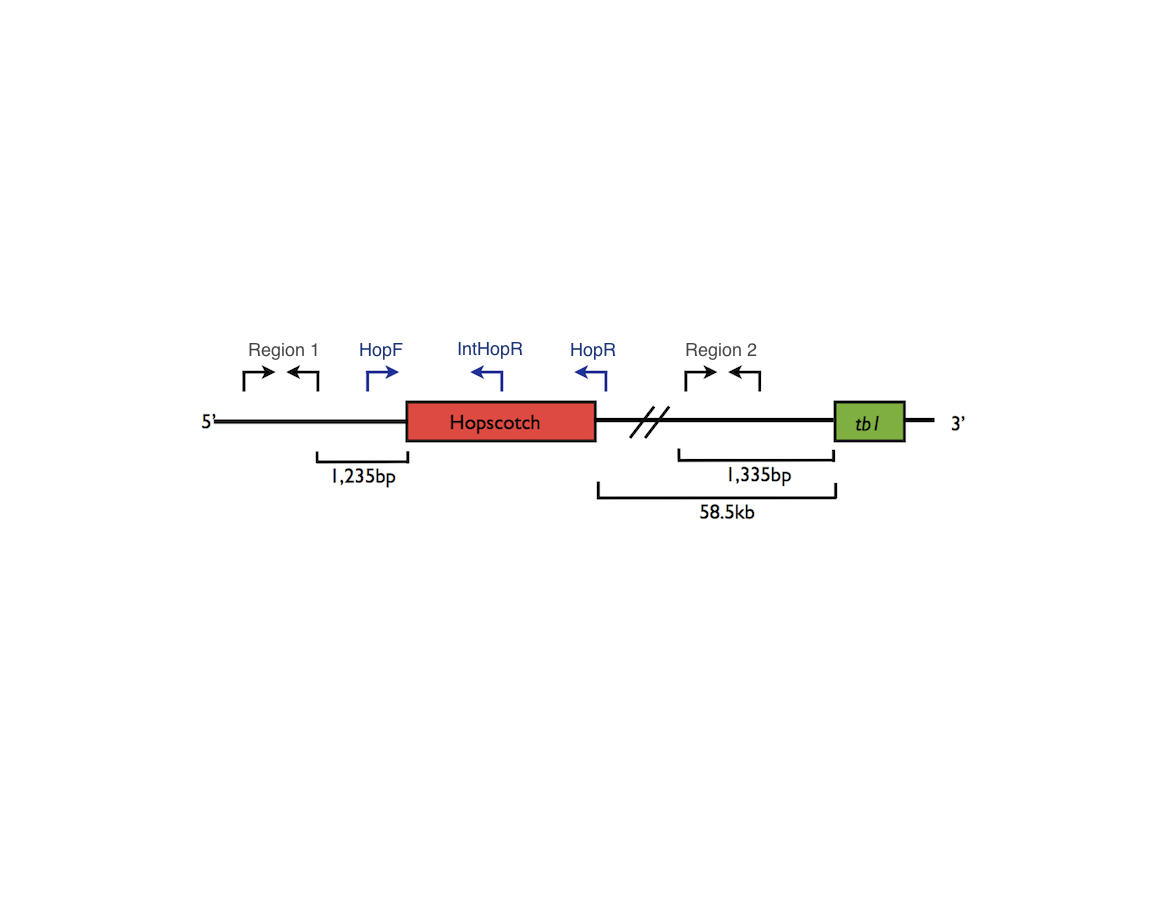
\includegraphics[width=180mm]{FigS1LocusCartoon.png}
   %\flushleft{Figure S1: Representation of the upstream regulatory region of \emph{tb1}, showing the \emph{tb1} coding region (green) and the \emph{Hopscotch} insertion (red). Arrows show the location of primer sets; in black, primers used for amplification and sequencing (Region 1; within the 5' UTR, and Region 2; 66,169 bp upstream from the tb1 ORF); in blue, primers used to genotype the \emph{Hopscotch} insertion.}
  %\end{center}
%\end{figure*}
%-------------------------------------------------------------------

\clearpage


% Appendix S4. Gel image
%-------------------------------------------------------------------
\begin{figure*}[!t]
  \begin{center}
   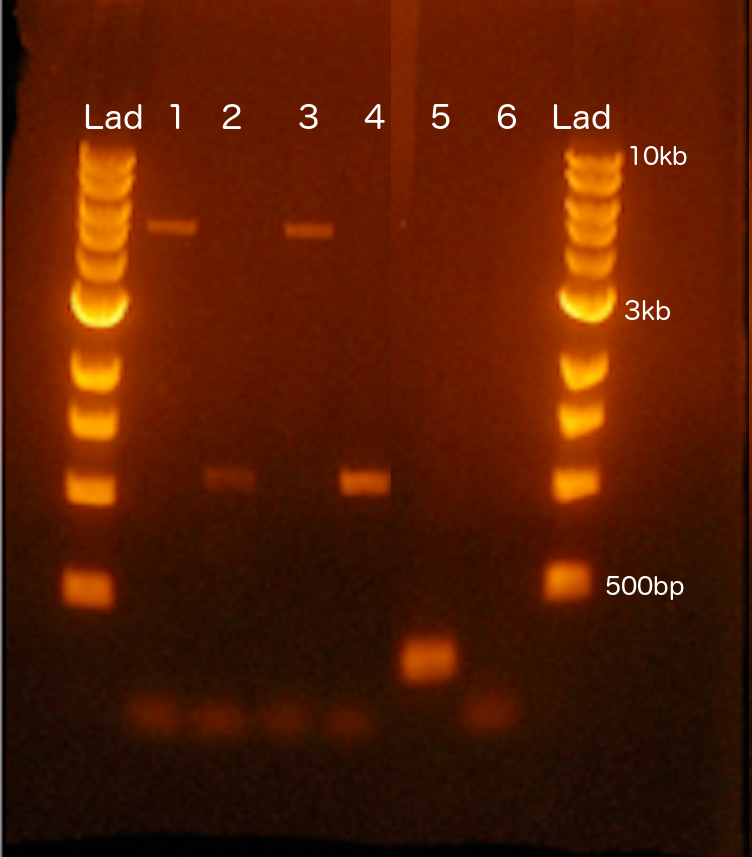
\includegraphics[width=100mm]{FigS2GelPeerJ_pretty.png}
   \flushleft{Figure S1: Agarose gel image of amplification products for genotyping of the \emph{Hopscotch} element. Lanes 1 (HopF/HopR; 5kb band) and 2 (HopF/HopIntR; 1.1kb) are the products for one individual that is homozygous for the element; Lanes 3 (HopF/HopR; 5kb band) and 4 (HopF/HopIntR; 1.1kb) are also the products of an individual that is homozygous for the element; and Lanes 5 (HopF/HopR; 300bp) and 6 (HopF/HopIntR; N/A) are the products of an individual that is homozygous for the teosinte (lacking the \emph{Hopscotch}) allele.} 
  \end{center}
\end{figure*}
%-------------------------------------------------------------------

\clearpage


% Appendix S5. NJ Trees
%-------------------------------------------------------------------
\begin{figure*}[!t]
  \begin{center}
   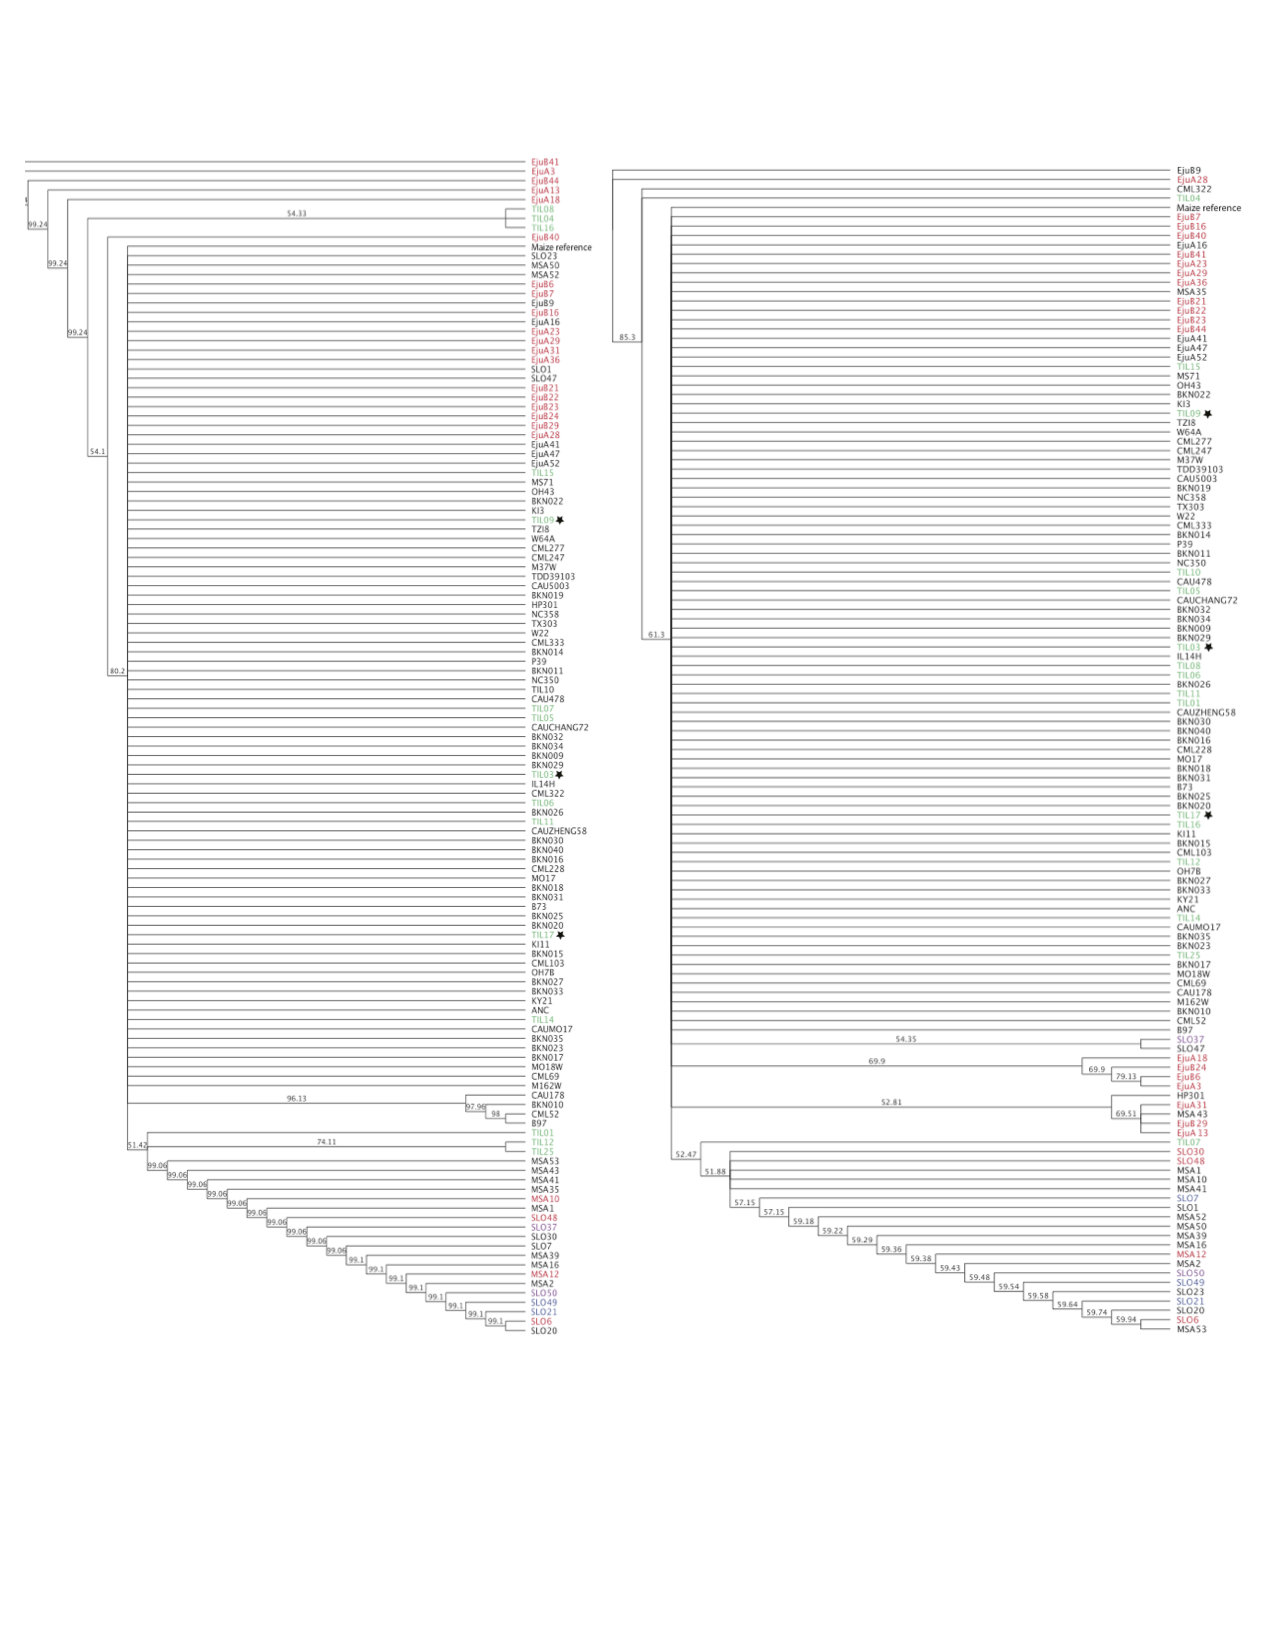
\includegraphics[width=150mm]{FigS3NJtrees.png}
    \flushleft{Figure S2: Neighbor-joining tree of the sequenced region in the 5' UTR (right; Region 1) and the 66,169 bp upstream region (left; Region 2) of \emph{tb1} using 10,000 bootstraps. Individuals with genotype data are colored: Homozygous for the teosinte (no \emph{Hopscotch}) allele (red), homozygous for the maize (\emph{Hopscotch}) allele (blue), heterozygotes (purple). TILs (teosinte inbred lines) are colored in green, with stars indicating the 3 TILs known to have the \emph{Hopscotch} insertion. Black indicates individuals not genotyped for the \emph{Hopscotch} insertion. EjuA refers to individuals from population Ejutla A, EjuB from Ejutla B, SLO from San Lorenzo, and MSA from La Mesa. Remaining individuals are lines of maize (\emph{Zea mays} ssp. \emph{mays}).}  

\end{center}
\end{figure*}
%-------------------------------------------------------------------
\end{document}
